\begin{mainquestion}{cstransfer}{Common Source Amplifier Transfer Characteristic}

Consider a common source (CS) amplifier as shown below. The key parameters are $V_{DD} = 10\ \text{V}$, $R_{D} = 3.4\ \text{k}\Omega$, $k_{n} = k_{n}^{\prime}\frac{W}{L} = 10\ \frac{\text{mA}}{V^{2}}$, and $V_{t} = 0.7\ \text{V}$. Assume $\lambda = 0$ for parts (a)-(d).

\begin{center}
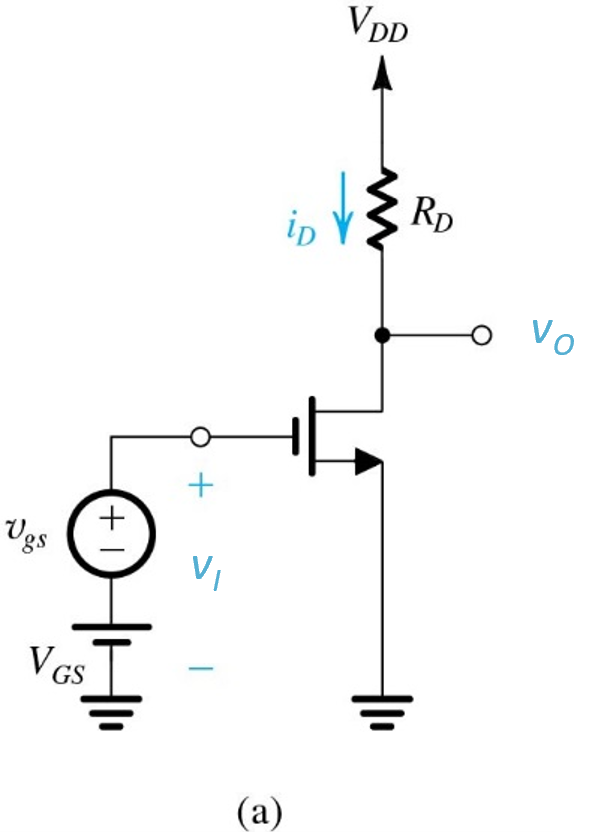
\includegraphics[width=2in]{../v0/Picture1.png}
\quad
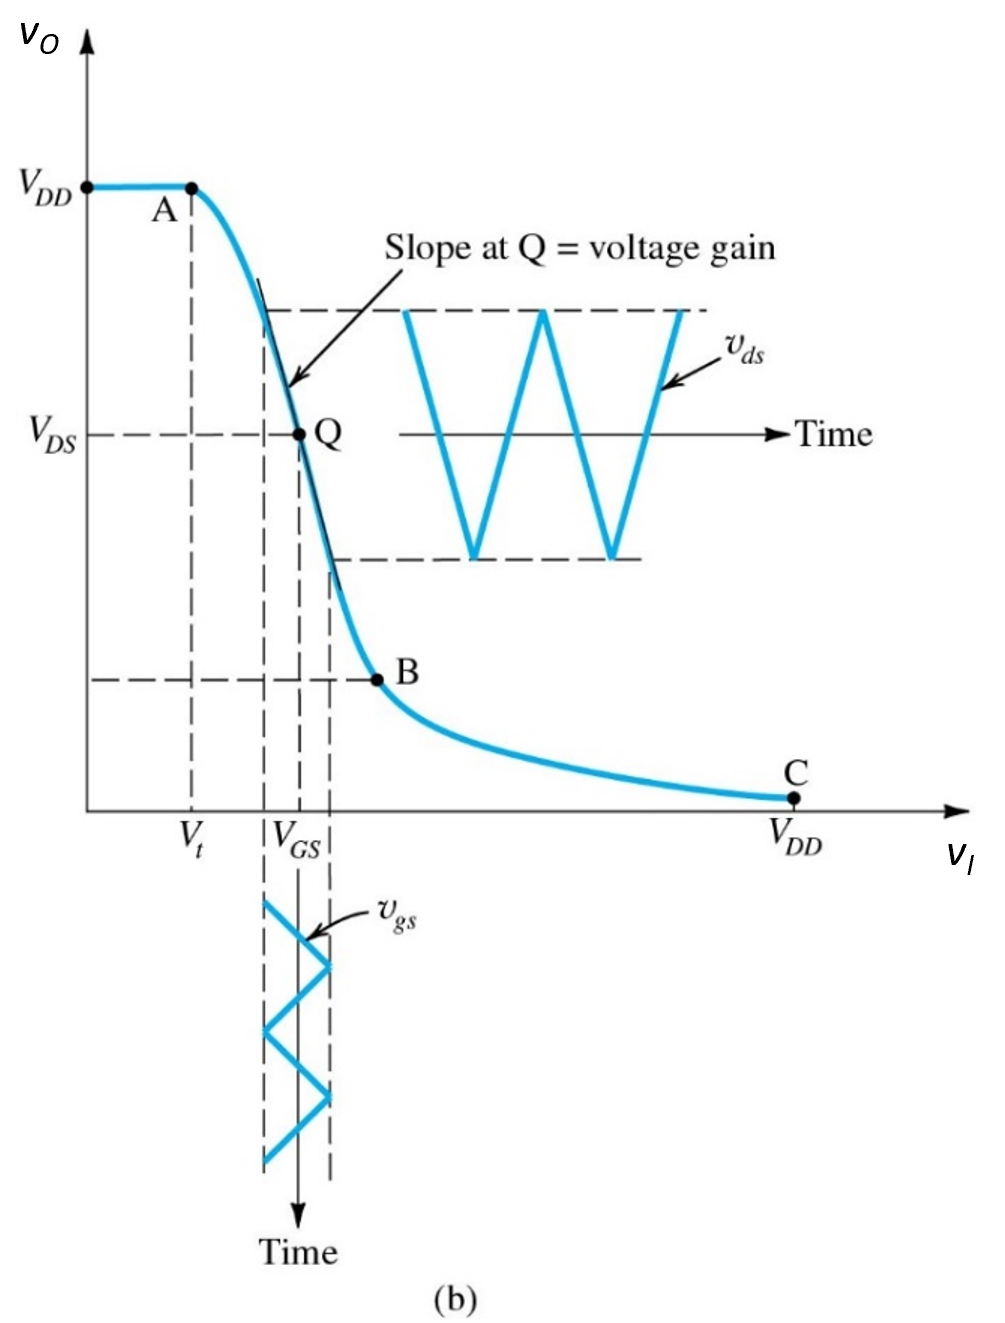
\includegraphics[width=3in]{../v0/Picture2.png}
\end{center}

\begin{partquestion}{findpointsab}{Find the coordinates of points A and B (i.e., $V_{I}$ and $V_{O}$) on the sketch in figure (b) above.}
\begin{answer}
\begin{kaitlyn}

\noindent\fbox{%
    \begin{minipage}{\dimexpr\textwidth-2\fboxsep-2\fboxrule\relax}
        \textbf{Why we're doing this problem:} Points A and B define the boundaries of the amplifier’s useful operating region, where the output looks like a scaled version of the input -- which is what we want: given some input signal, predict what signal comes out!
    \end{minipage}%
}



\end{kaitlyn}
Point A on the sketch corresponds to the moment when the transistor transitions from cut-off to saturation. This occurs when $v_{I} = v_{GS} = V_{t} = 0.7\ \text{V}$. At this point, current is just beginning to flow so $v_{DS} = v_{O} = V_{DD}$. So, point A is (0.7 V, 10 V).

Point B corresponds to the moment where the transistor goes from saturation to triode. In this case, $V_{DS} = V_{GS} - V_{t}$ so $v_{O} = v_{I} - V_{t} = v_{I} - 0.7\ \text{V}$. Because at point B we are at the boundary of two regions, either formula for $I_{D}$ should work (also because $\lambda = 0$, which ensures continuity between regions with our standard formulas for $I_{D}$). Choosing that of saturation gives:

\[
I_{D} = \frac{V_{DD} - v_{O}}{R_{D}} = \frac{1}{2} k \left(V_{GS} - V_{t}\right)^{2}
\]

so

\[
\frac{10 - v_{O}}{3.4} = \frac{1}{2}(10)(v_{I} - 0.7)^{2} = \frac{1}{2}(10)v_{O}^{2}
\]

this leads to the quadratic:

\[
5 v_{O}^{2} + 0.2941 v_{O} - 2.9412 = 0
\]

which has solutions $v_{O} = -0.797$ and $v_{O} = 0.738$. Only the second is a valid solution. From here, $v_{I} = v_{O} + 0.7 = 1.438\ \text{V}$, so point B is (1.438 V, 0.738 V).

\begin{kaitlyn}

\textbf{Zooming out:} We’re moving one level higher in abstraction: zooming out from the MOSFET as an individual device to the MOSFET as an amplifier. The same $V_{GS}$, $V_{DS}$, and $I_{D}$ and region-of-operation tools still apply from previous lectures, but now we use them to understand the circuit-level relationship between $v_O$ and $v_O$. Ultimately, that is what we want from an amplifier: given some input signal, predict what signal comes out. Once we understand this input-output behavior, we can characterize the amplifier by parameters like gain, $R_i$, and $R_o$, and eventually treat the entire amplifier as a building block in a larger circuit.

    
\end{kaitlyn}


    
\end{answer}
\end{partquestion}

\begin{partquestion}{biaspoint}{If the amplifier is biased to operate with an overdrive voltage $V_{OV} = V_{GS} - V_{t} = 0.5\ \text{V}$, find the bias point Q on the transfer characteristic. What is the value of $I_{D}$ when operating at the bias point Q?}
\begin{answer}
We know with this overdrive voltage level:

\[
v_{I} = V_{GS} = V_{OV} + V_{t} = 0.5 + 0.7 = 1.2\ \text{V}.
\]

We can use the same equation as in part (a) to find the output voltage:

\begin{gather*}
    \frac{10 - v_o}{3.4} = \frac{1}{2}(10)(v_I - 0.7)^2 = \frac{1}{2}(10)v_{OV}^2 = 5(0.5)^2 = 1.25 \\
    v_o = 10 - (1.25)(3.4) = \qty{5.75}{\volt}
\end{gather*}

The point Q is therefore (1.2 V, 5.75 V). It follows that:

\[
I_{D} = \frac{10 - v_{O}}{3.4} = \frac{10 - 5.75}{3.4} = \qty{1.25}{\milli\ampere}.
\]
\end{answer}
\end{partquestion}
\begin{partquestion}{maxamplitude}{At the bias point Q, what is the largest amplitude of a sine-wave voltage signal that can be applied at the input while the transistor remains in saturation? What is the peak-to-peak voltage of the output signal that results?}
\begin{answer}

\begin{kaitlyn}

    Beginning with our DC bias point:
    \begin{align*}
        (\qty{1.2}{\volt}, \qty{5.75}{\volt})
    \end{align*}
    
    we need to consider the AC time-varying component 
    \begin{align*}
        v_I(t) = V_{GS} + v_{gs}(t)
    \end{align*}
    

    and how big a signal $v_{gs}$ can be applied before it pushes the transistor out of saturation regime.

    We know that anything beyond our previously-found bounds, point A (\qty{0.7}{\volt}, \qty{10}{\volt}) and point B (\qty{1.438}{\volt}, \qty{0.738}{\volt}), would push the transistor out of saturation. 

    (If it helps, try drawing out a simple sine wave to help visualize, making sure it's offset at \qty{1.2}{\volt}, and seeing which bound you hit first, \qty{1.438}{\volt} or \qty{0.7}{\volt} from \qty{1.2}{\volt}!) 

    
\end{kaitlyn}
Since our quiescent point Q has an input voltage which is closer to point B's input voltage than it is to point A's input voltage, a sine wave centered on point Q (about \qty{1.2}{\volt}) will hit a limiting point at B (\qty{1.438}{\volt}) when its amplitude is $1.438 - 1.2 = \qty{0.238}{\volt}$. 
\begin{kaitlyn}
    \begin{figure}
        \centering
        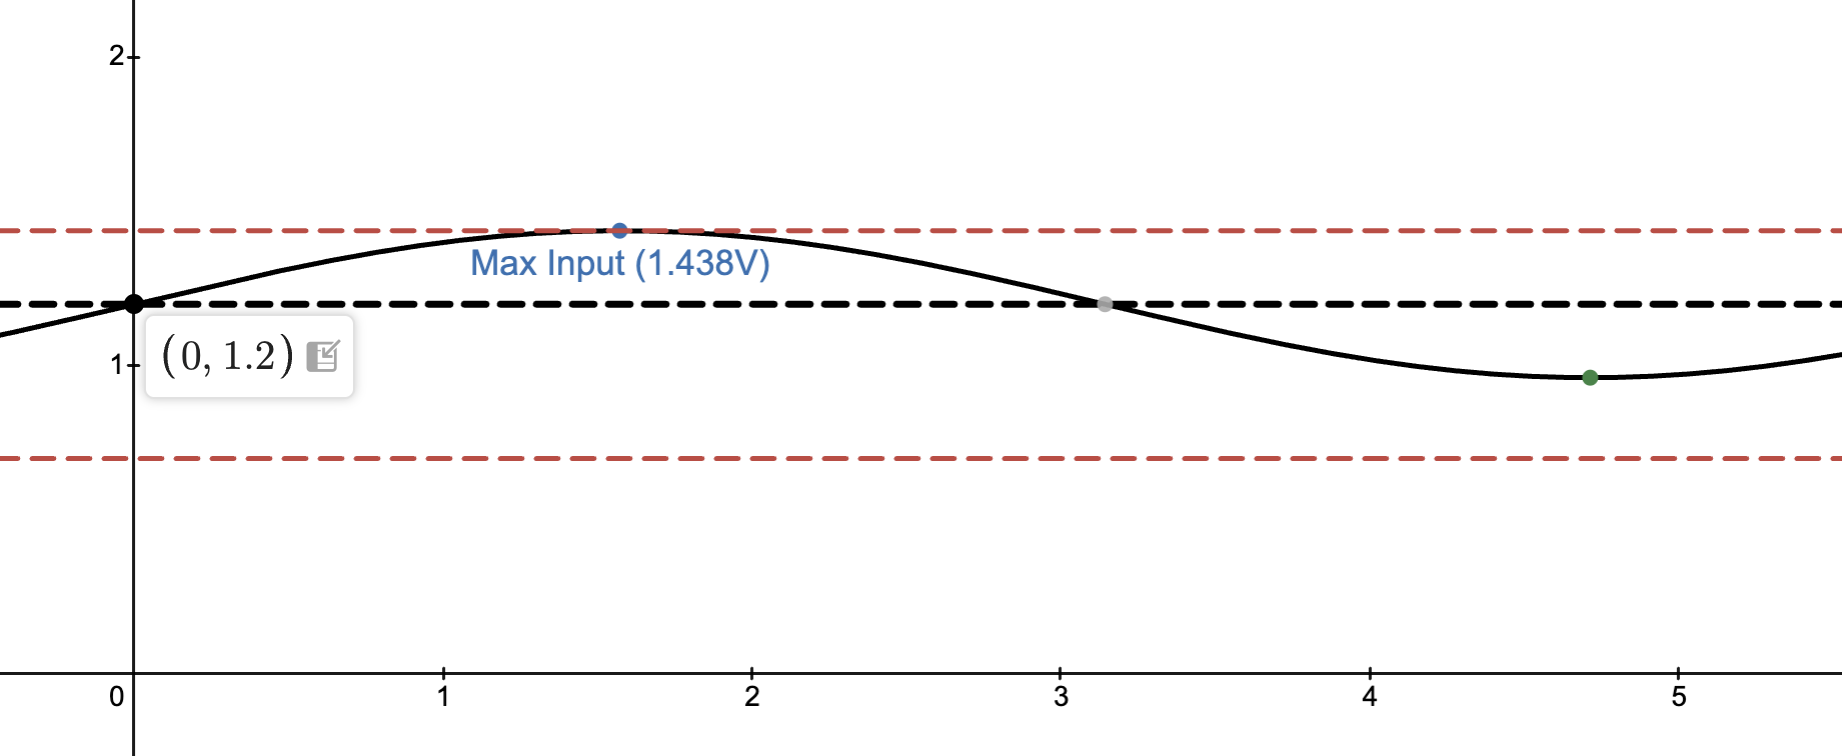
\includegraphics[width=0.5\linewidth]{sine_swing_limits.png}
        \label{fig:cstransfer:sineswing}
    \end{figure}
\end{kaitlyn}
While there will be distortion due to the square-law relationship of the current in the saturation regime, it will remain in saturation. With an input sine wave of amplitude of \qty{0.238}{\volt}, at the maximum input, the output will dip to \qty{0.738}{\volt} (since we are touching point B). 

At the minimum input, the output will rise to a value determined by an input $v_{I} = 1.2 - 0.238 = \qty{0.962}{\volt}$ as follows:
\begin{align*}
    \frac{10 - v_O}{3.4} &= \frac{1}{2}(10)(v_I - 0.7)^2 \\
    10 - v_O &= (5)(3.4)(0.962 - 0.7)^2 \\
    v_O &= 10 - (5)(3.4)(0.962 - 0.7)^2 \\
    &= \qty{8.83}{\volt}
\end{align*}

The peak-to-peak voltage of the output signal is then $8.83 - 0.738 = \qty{8.095}{\volt}$.


\begin{kaitlyn}
    \noindent\fbox{%
    \begin{minipage}{\dimexpr\textwidth-2\fboxsep-2\fboxrule\relax}
        \textbf{Developing Intuition:} Real signals that go into systems are rarely ever clean DC voltages (ex: a microphone, antenna will produce a voltage that changes with time). Since we know the bounds in which the amplifier circuit will operate in its linear regime (through MOSFET saturation equations), we can then determine how large an AC signal input can be for our specific system. But actually, usually circuit designers work the other way: they are given an AC amplitude spec and they design their system to be able to meet it.
    \end{minipage}%
    }
\end{kaitlyn}

\end{answer}
\end{partquestion}

\begin{partquestion}{gainandtransconductance}{What are the transconductance $g_{m}$ and gain $A_{v}$ at point Q? Provide the gain both in linear (V/V) and log (dB) units.}
\begin{answer}


The transconductance is:

\begin{align*}
    g_m &= k(V_{GS} - V_t) \\
    &= 10(1.2 - 0.7) \\
    &= \qty{5.0}{\milli\siemens}
\end{align*}

The gain (ignoring output resistance) is:

\[
A_{vo} = -g_{m} R_{D} = -5(3.4) = -17\ \frac{\text{V}}{\text{V}}
\]

which, in decibels is:

\[
A_{vo,\text{dB}}= 20\log|A_{vo}| = 20\log|17| = 24.6\ \text{dB}.
\]

\end{answer}
\end{partquestion}

\begin{partquestion}{lambdaeffect}{Now consider the MOSFET has a non-zero channel-length modulation parameter $\lambda$. What is the maximum $\lambda$ allowed so the voltage gain does not fall below 24 dB? What is the minimum output resistance $r_{o}$? (You may assume the bias point Q is not affected by $\lambda$.)  }
\begin{answer}

\begin{kaitlyn}
    \noindent\fbox{%
    \begin{minipage}{\dimexpr\textwidth-2\fboxsep-2\fboxrule\relax}
        \textbf{What we're really answering:} MOSFETs are not ideal. How much MOSFET non-ideality can we tolerate before the entire amplifier fails to meet its required gain?
    \end{minipage}%
    }

    
\end{kaitlyn}

\begin{kaitlyn}


 Until now, we assumed $\lambda=0$, meaning our MOSFET behaved like an ideal current source in saturation. Once $V_{GS}$ set $I_D$, changing $V_{DS}$ did not change the drain current:


 \[\lambda=0 \qquad \Longrightarrow \qquad r_o=\infty.\]

Real MOSFETs are not ideal current sources. Due to \textbf{channel-length modulation}, increasing $V_{DS}$ causes $I_D$ to increase slightly even when the transistor remains in saturation. This is why the saturation-region $I_D$--$V_{DS}$ curves are not perfectly flat.

We capture this non-ideality in the small-signal model with

\[r_o=\frac{1}{\lambda I_D}.\]

A larger $\lambda$ therefore means a smaller $r_o$: the MOSFET behaves less like an ideal current source.


\textbf{Follow the figure on the next page with the small signal model drawn out and how it fits back into the larger circuit!}

\begin{figure}
    \centering
    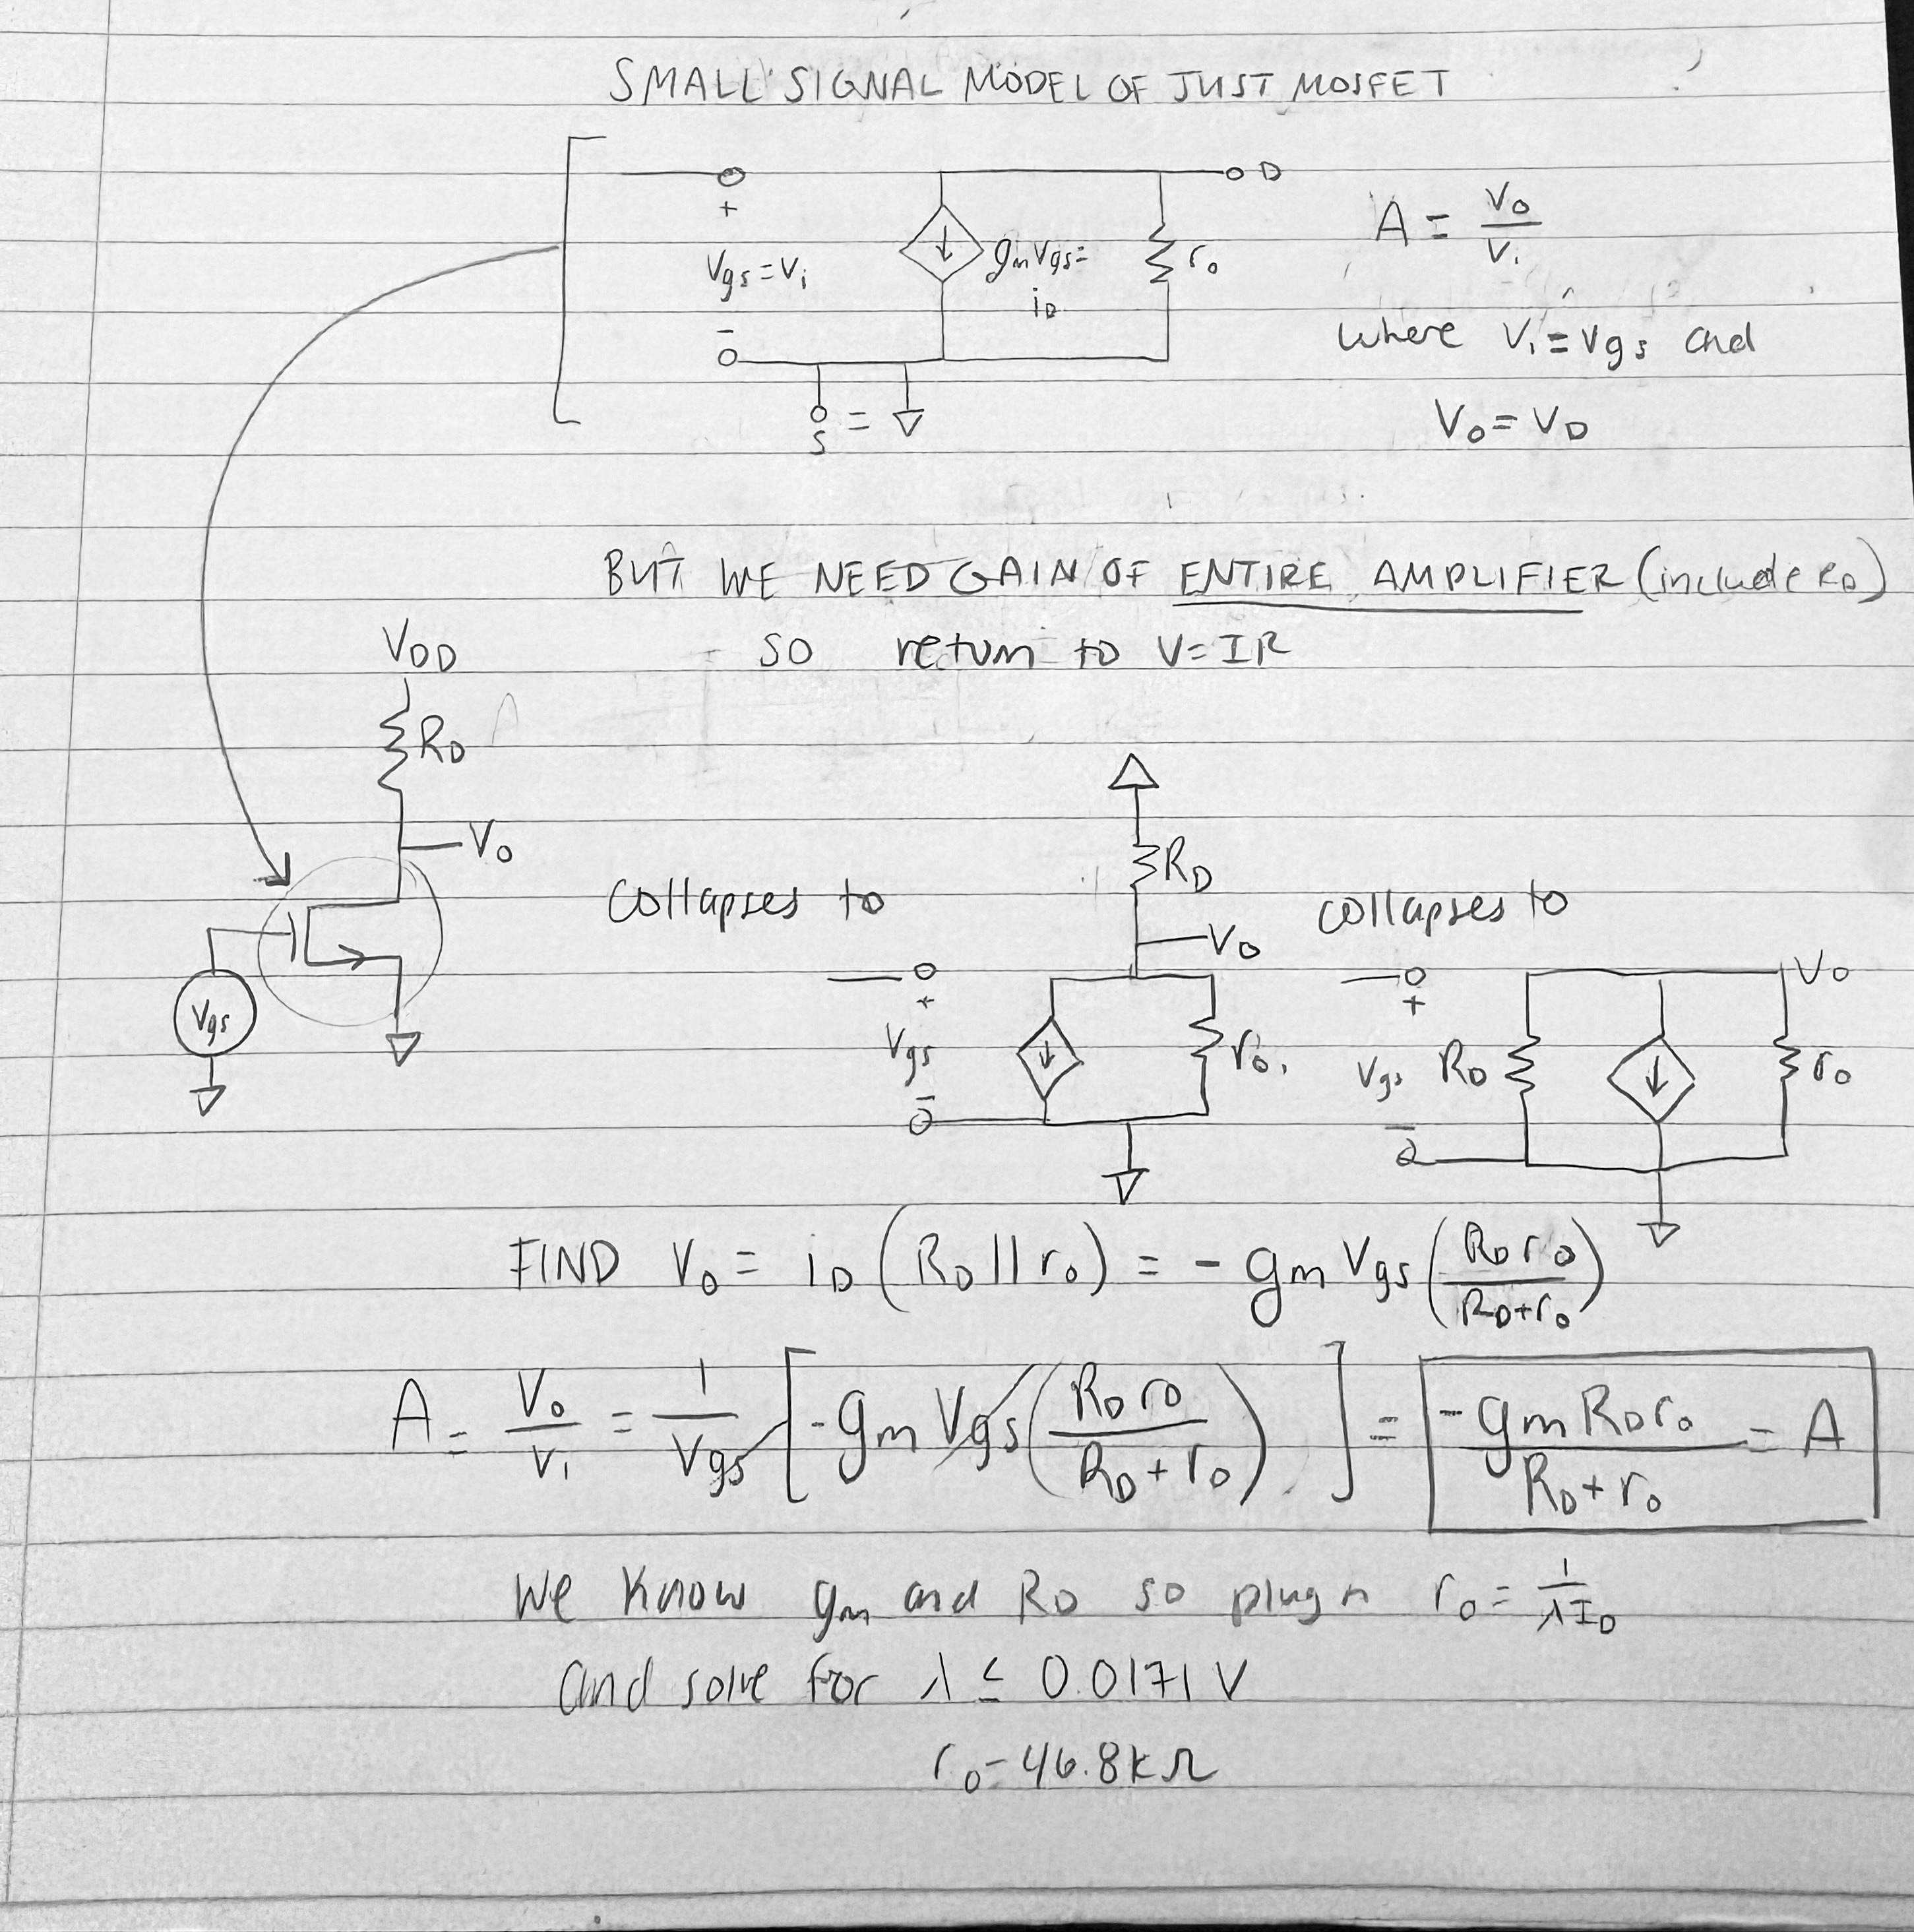
\includegraphics[width=1\linewidth]{small_signal_ro_notes.jpeg}
    \label{fig:cstransfer:smallsignalnotes}
\end{figure}
$r_o$ belongs to the small-signal model of the MOSFET, but the MOSFET is only one part of our common-source amplifier. When we put its small-signal model back into the complete circuit, $V_{DD}$ becomes AC ground, so both $R_D$ and $r_o$ connect from the output node to ground. Thus, the current $g_m v_{gs}$ sees

\[R_D \parallel r_o,\]

and the amplifier gain becomes

\[A_v=-g_m(R_D\parallel r_o)\]

rather than the ideal result $A_v=-g_mR_D$.
\end{kaitlyn}

With output resistance, the formula for the gain is modified slightly:

\[
A_{vo} = -g_{m} \left(R_{D} \parallel r_{o}\right) = -\frac{g_{m} R_{D} r_{o}}{R_{D} + r_{o}}
\]

Because the minimum gain must be 24 dB, we have:

\begin{align*}
    20\log|A_v| &\geq 24 \\
    20\log\left(\frac{g_m R_D r_o}{R_D + r_o}\right) &\geq 24 \\
    \left(\frac{g_m R_D r_o}{R_D + r_o}\right) &\geq 10^\frac{6}{5} \\
    g_m R_D r_o &\geq 10^\frac{6}{5}R_D + 10^\frac{6}{5}r_o \\
    r_o &\geq \frac{10^\frac{6}{5}R_D}{g_m R_D - 10^\frac{6}{5}} \\
\end{align*}

Since $r_{o} = \frac{1}{\lambda I_{D}}$, we have:

\begin{align*}
    \lambda &= \frac{1}{r_o I_D} \\
    &\leq \frac{g_m R_D - 10^\frac{6}{5}}{10^\frac{6}{5}R_D I_D} \\
    &\leq \frac{(5) (3.4) - 10^\frac{6}{5}}{10^\frac{6}{5}(3.4)(1.25)} \\
    &\leq \qty{0.0171}{\per\volt} \\
\end{align*}

so, it follows that

\[
r_{o} \geq \frac{1}{\lambda_{\max} I_{D}} = \frac{1}{(0.0171)(1.25)} = 46.8\ \text{k}\Omega.
\]

\begin{kaitlyn}
    \noindent\fbox{%
    \begin{minipage}{\dimexpr\textwidth-2\fboxsep-2\fboxrule\relax}
        \textbf{Why we're doing this problem:} This is where it got tricky. We're bridging our individual MOSFET model to a higher-level, larger circuit model, specifically the common-source amplifier circuit. You should be able to generalize small-signal models and derive gain for any new circuit, from ideal CS amplifiers to new configurations with non-idealities.
    \end{minipage}%
    }
\end{kaitlyn}
\end{answer}
\end{partquestion}

\end{mainquestion}
